% DNS defined in the intro!
\subsection{Incompressible DNS Application}
\label{sec:dns_full}

% Why DNS code needs to be improved
Direct numerical simulation (DNS) plays an important role in understanding turbulent flows because DNS provides high fidelity data that is difficult to obtain in the experiments. After Kim {\it et al.} first used the DNS for wall-bounded turbulence flow in 1987 \cite{Kim:1987ub}, DNS has been used extensively to understand the turbulence phenomenon and to help develop models of turbulence. In general, the length-scale and time-scale become smaller as $Re$ increases where $Re$ is Reynolds number. Natually, DNS at high $Re$ requires a large number of grids and time-steps to obtain meaningful statistical data. Therefore, the use of state-of-art HPC system is crucial to study the turbulent flow of high Re. To date, the highest $Re$ of the wall-bounded turbulence DNS is 250000, for which 242 billion degrees of freedom are used. \cite{Lee:2015er} However, $Re$ = 250000 is also low compared to the high Re flow required for many practical engineering applications. For a DNS at higher Re, more advanced HPC system is required, and the DNS code should also be improved for the the HPC system.

% Detail of simulation
In this section, we will show you the results of testing PoongBack on KNL nodes in Stampede, which is a channel flow DNS code optimized for the modern HPC systems. PoongBack simulates the flow between two parallel plates with periodic boundary conditions. The simulation code has already shown excellent performance and has been already used in several researchers. \cite{Lee:2013kv} Especially, it has been used for generating the data for virtual flow laboratory in Johns Hopkins Turbulence Data Base \cite{Graham:2015ha}.It is using Fourier-Galerkin method in streamwise direction and high order basis spline method in wall-normal directions. For time integration PoongBack uses low-storage third order Runge-Kutta method. The simulation domain is partitioned by two-dimensional decomposition, a.k.a. pencil-decomposition. PoongBack contains three major kernels; (1) solving Navier-Stokes equation in complex number domain (2) one-dimensional fast Fourier transforms in real-to-complex, complex-to-real and complex-to-complex (3) data transpose in two dimension. The combination of (2) and (3) makes 3D FFT and there are multiple libraries for it. We developed customized 3D FFT library because of the needs of zero-padding for 3/2 dealiasing. Additionally, PoongBack uses customized I/O library for HDF5 format, ESIO \cite{Lee:2014ta}, but the I/O performance is not the scope of current work. See \cite{Lee:2013kv,Lee:2014ta} for more detail about PoongBack.  

\begin{figure}[htb]
 \begin{center}
   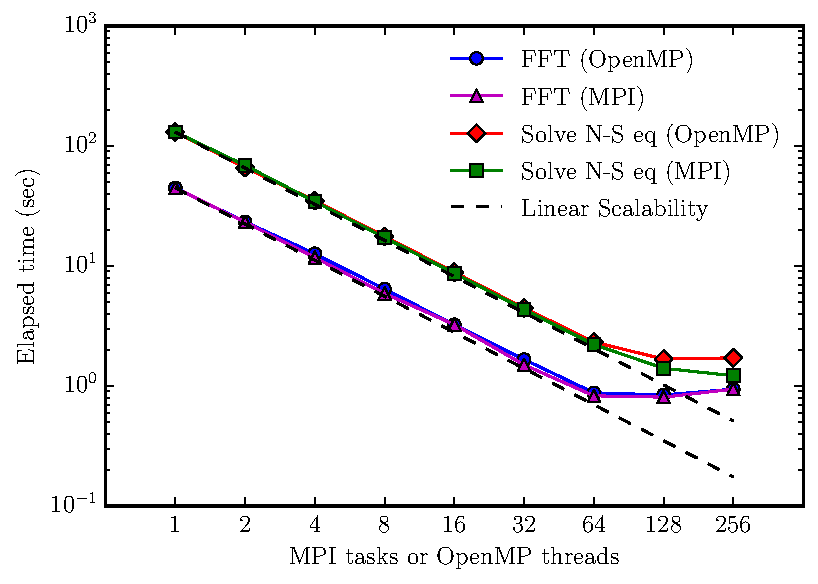
\includegraphics[width=0.45\textwidth]{DNS_FFT_Wave}
   \caption{Strong scaling result of 1D FFTs and Solving N-S equations in wavespeace for single timestep.}
   \label{fig:DNS_strong_scale_fft_wave}
 \end{center}
\end{figure}

% 1D FFT and wavespace performance

For this study the grid size is used $1024\times128\times512$ and the grid size is comparable for $Re_\tau = 180$ simulation by \cite{Kim:1987ub}. Throughout the every benchmark cases, the MCDRAM is used as a cache memory between processors and DRAM. Figure~\ref{fig:DNS_strong_scale_fft_wave} shows the strong scaling performance of 1D FFTs (real-to-complex, complex-to-real and complex-to-complex) and floating point operations with complex numbers including linear equation solvers. The linear equation, $A\mathbf{x} = \mathbf{b}$, is solved to compute B-spline coefficients. $A$ is a diagonal dominant banded matrix with additional non-zero elements in several top and bottom rows. $\mathbf{x}$ and $\mathbf{b}$ is complex vectors. As shown in the Figure~\ref{fig:DNS_strong_scale_fft_wave}, FFTs and floating point operations shows good scalability in both OpenMP only and MPI only cases with upto 64 processors. Using MPI only shows slightly better performance but the difference is negligible. After the hyperthread\todo{it this right term?} is used performance with FFTs are decreased because FFTs are bounded by the memory access not by floating point operations. On the otherhands, the kernel with linear equation shows slight performance increases even with the hyperthreads. Interestingly, using MPI shows better performance than OpenMP. This maybe due to the difference of memory access pattern between two parallelism. \todo{Chris, is this make sense?}.

% Transpose performance

\begin{figure}[htb]
 \begin{center}
   \includegraphics[width=0.45\textwidth]{DNS_Transpose}
   \caption{Strong scaling result of data reorder and MPI communication; OpenMP is not used.}
   \label{fig:DNS_strong_scale_transpose}
 \end{center}
\end{figure}

% Full timestep performance

\begin{figure}[htb]
 \begin{center}
   \includegraphics[width=0.45\textwidth]{DNS_Parallelism}
   \caption{Comparison of MPI$\times$OpenMP configuration}
   \label{fig:DNS_MPI_OpenMP}
 \end{center}
\end{figure}

\begin{figure}[htb]
 \begin{center}
   \includegraphics[width=0.45\textwidth]{DNS_full_timestep}
   \caption{Strong scaling result of total elapsed time for single timestep; (MPI tasks $\times$ OpenMP threads) is hybrid configuratation which showed  the best performance.}
   \label{fig:DNS_strong_scale_total_elapsed_time}
 \end{center}
\end{figure}





\todo{if we merge this with the previous section, we can have an intro
to dns and then talk about each in detail}

